\pagenumbering{arabic}
\chapter{Introduction}

%With this thesis consisting of two disparate and apparently unrelated subjects I hope to begin with a common introduction that underlies both subjects collectively. The issue of neutral particle detection is one that is very problematic and concerns both LAGUNA-LBNO and MODES-SNM. The use of noble gas detection however is key to their detection with Argon being the most prevalent in modern technologies. 

The issue of neutral particle detection is one that can be very problematic and concerns both LAGUNA-LBNO and MODES-SNM. Photons, neutrons and neutrinos collectively form the family of particles of interest. They are introduced sequentially in this chapter to motivate their relevance in these two disparate and apparently unrelated projects.

%%Neutral Particles
\section{Neutral Particles}
Particles pertaining no net electrical charge are considered neutral. Neutrons, gammas and neutrinos are all stable or long-lived neutral particles. Although their difficulty in detection can be troublesome it is also what makes them very attractive to study. This family of particles will not leave tracks in ionisation detectors and poses the ability to pass through materials unscathed.  Such a property is useful for monitoring systems that cannot be physically examined and allows for non intrusive methods in detection. Examples of this are reactor monitoring using neutrinos \cite{neutrinoReactorMonitoring} and radiation monitoring using neutrons and gammas \cite{website:modes}. The former is a modern idea proposed and proof of concept has been shown, with the latter very much the focus of this thesis.

\section{The Photon}
The idea of the photon arose on the turn of the 20$^{th}$ century when Max Planck was working on blackbody radiation. He coined the term `energy elements' \cite{maxPlanckPackets} to describe electromagnetic waves released in energy packets. Planck found that quantising the radiation in such a way, the energy, $E$, was proportional to the frequency of the radiation, $\nu$, equation~\ref{eq:photonEnergy}. The constant of proportionality, Planck's constant, is $h$ = 6.63 $\times$ 10$^{-34}$ Js. 

\begin{equation}
E = h\nu
\label{eq:photonEnergy}
\end{equation}

It was not until 1905 that it was understood why this happened to be the case, when Einstein put forward his idea, stemming from Planck's initial findings \cite{einsteinQuanta}. He suggested it was an inherent property of the electromagnetic radiation itself, opposed to Plancks emission process idea. In turn this led Einstein to the Nobel Prize in 1921 for an explanation of the photoelectric effect. Following this revelation a further publication in 1909 justified that these light quantum should be considered as particles themselves \cite{einsteinPhoton}. 

%In this process electrons are emitted from a metal surface upon electromagnetic radiation striking it.

Arthur Compton confirmed Einstein's theory and his controversial claims in 1923 with his work on X-ray scattering off light elements \cite{compton}. For an incident wavelength $\lambda$, on a target of mass $m$, scattered through an angle $\theta$, with final wavelength $\lambda^{'}$, he found that this shift was in accordance with equation~\ref{eq:compton}. The Compton wavelength of the target particle is then $\lambda_{c} = h/mc$. Kinematically this is equivalent to a particle of zero rest mass, thus confirming that light can carry momentum and hence behaves as a particle with zero rest mass.

\begin{equation}
\lambda^{'} - \lambda =  \frac {h}{mc} (1 - cos\theta)
\label{eq:compton}
\end{equation}
 
The name, photon, is accredited to chemist Gilbert Lewis \cite{photonName} and since becoming a well established particle, it has opened up our view on the physical world and helped forge Quantum Field Theory. The photon is now considered as a quantum of light.
 
\subsection{Gamma Radiation}
Photons of energy > 100 keV are considered gamma rays. Such energies correspond to extremely high frequencies of the order 10$^{10}$ GHz and above. In many nuclear gamma emissions energies are of the order of 1 MeV, corresponding to a wavelength of $\sim$1.2 pm. This distance is extremely small, much smaller than the radius of an atom and for energies exceeding 1 GeV it is comparable with the radius of the nucleus. Gamma emission can arise from many radiative processes, it is useful to discuss the key types.

\subsubsection{Nuclear Transition Radiation}
Gamma ray emission can occur through the excitation of nuclei and the subsequent transition to a lower nuclear energy state, with the energy of the photon equal to the difference between energy levels. Radionuclides can decay in several ways but most processes will leave the nucleus in an excited state. Although these processes can have large half-lives the de-excitation happens very quickly, over the order of picoseconds. Due to this process the energy spectrum of the gamma radiation gives an indication of the energy structure of the daughter nucleus while the rate gives an indication of the half-life of the parent nucleus. As nuclear energy levels are discrete and well defined this can yield almost mono energetic gamma rays, making their sources perfect candidates for the energy calibration of detectors. $^{60}$Co is a perfect example of this, as it decays via  $\beta$-decay leaving the nucleus in an excited state. Upon de-excitation of the remnant $^{60}$Ni, two photons of 1.173 and 1.332 MeV respectively are emitted every time \cite{knollRadiation}.

\subsubsection{Annihilation Radiation}
In the case when a positron is emitted, under $\beta^{+}$ decay, it will usually annihilate with a  electron in a nearby atom once it has lost its kinetic energy. This will then produce two photons equal in energy and opposite in direction, each with energy of $m_{e}$ = 0.511 MeV. Annihilation radiation generally occurs with other radiative processes and will be superimposed in the spectrum.

\subsubsection{Bremsstrahlung Radiation}
Accelerating charged particles produce electromagnetic radiation. An electron passing through matter will interact electromagnetically with the material and thus radiate. This is Bremsstrahlung radiation. Unlike nuclear de-excitation, Bremsstrahlung radiation yields a continuous energy spectrum and is not useful for energy calibration of detectors. 

\subsection{Interactions}
Gamma rays interact via three main processes: Photoelectric Absorption, Compton Scattering and Pair Production. Their interaction probabilities are then proportional to Z$^{5}$/$E^{7/2}$, Z/$E$ and Z$^{2}$ln(2$E$) respectively \cite{nobleGasDetectors}, where Z is the atomic number of the material and $E$ is the incident gamma energy. This then describes the dominant processes in ascending order of gamma energy, with the photoelectric absorption dominating at low energies, Compton scattering at intermediate energies and then pair production dominating at energies above 2$m_{e}$ = 1.022 MeV.

\subsubsection{Photoelectric Absorption}
Photoelectric absorption involves the complete conversion of a photon to an energetic electron. The photon will interact with the absorber atom as a whole and cannot occur with the electrons in the bound shell. When the photon is absorbed a photoelectron is emitted from one of the bound shells on the atom. The most probable shell origin for such a photoelectron is the K shell, the most tightly bound shell of the atom. The kinetic energy of the photoelectron is simply,

\begin{equation}
E_{e} = h\nu - E_{0}
\end{equation}
where $E_{0}$ represents the binding energy of the electron in its shell. Due to conservation of momentum however some energy is lost to nuclear recoil, but such considerations are negligible.

With binding energies of the order of $\sim$40 keV for the K shell in Xenon \cite{nobleGasDetectors}, when the incident gamma energy exceeds a few hundred keV, the photoelectron gives a good indication of the original gamma energy. It is therefore an ideal process when concerned with measuring the energy spectrum of gamma sources.

\subsubsection{Compton Scattering}
Kinematic restrictions infer that a Compton scattered photon will produce an electron with kinetic energy 
\begin{equation}
E_{e} = h\nu - h\nu^{'} = h\nu\Bigg[\frac{h\nu/m_{e}(1-\cos{\theta})}{1 + h\nu/m_{e}(1-\cos{\theta})}\Bigg], 
\label{eq:compton2}
\end{equation}
following from equation \ref{eq:compton}. Therefore a continuum of energies result from a mono energetic gamma ray due to the scattering angle $\theta$, for which any angle can occur. In the extreme case of shallow grazing ($\theta$ $\sim$ 0) then $E_{e}$ $\sim$ 0 and no interaction is observed. For the other case when maximum scattering occurs ($\theta$ = $\pi$), i.e backscattering, the incident gamma cannot transfer all of its energy to the electron and a Compton edge can be seen in the electron energy distribution. Only at energies well exceeding $h\nu$ $\gg$ $m_{e}/2$ can it be considered very close to the incident gamma energy.

\subsubsection{Pair Production}
As gamma energies reach several MeV pair production becomes the dominant process. In pair production the entire photon is converted to an electron and positron pair due to the intense electric field of the protons in the absorber nuclei. Once the energy threshold of 2$m_{e}$ is exceeded then the process in energetically viable and the total kinetic energy of the pair is then

\begin{equation}
E_{e^{+}} + E_{e^{-}} = h\nu - 2m_{e}.
\end{equation}

The emitted electron positron pair will only travel a short distance, losing all their kinetic energy to the absorbing material. The positron will come to rest, comparable to the thermal energy of the electrons in the material, and subsequently annihilate with such an electron. Annihilation results in the emission of two photons, each of energy 511 keV = $m_{e}$, with opposite and equal momenta due to conservation laws. 

\section{The Neutron}
It was in 1920 when Ernest Rutherford first introduced the notion of the neutron \cite{rutherfordNeutron} to explain the discrepancy between the atomic mass and the atomic number of the atom. It also introduced the rational to explain the prevention of the positively charged protons in the nucleus from repelling each other. After some years of considering that this could actually be due to nuclear electrons, the proton-electron nuclear model was rejected subject to proof by V. A. Ambartsumain and D. Ivanenko \cite{protonElectronNuclearModel}. Deducing that a neutral particle must also exist in the nucleus. It was not until twelve years after Rutherford first theorised the neutron that it was confirmed by James Chadwick \cite{Chadwick}. This discovery had enormous and explosive implications to modern society, introducing threats that are still very much imminent today.

With the ability to traverse many centimetres of dense materials they can be very difficult to detect. Neutrons can interact in a manner of ways but the three main processes of concern are; elastic scattering, inelastic scattering causing an excited nuclear state and absorption. It is considered useful to divide neutrons into two categories, slow (thermal) and fast, as certain interactions are favourable in these two classes.
%Neutrons can interact indirectly to produce charged particles which can then be easily detected. 
\subsection{Slow Neutrons}
Neutrons with kinetic energies of $\sim$0.5 eV and below are considered slow neutrons. Although this definition is not exact, it is used as a rough approximation to define the transition from fast to slow neutrons. At room temperature, $\sim$300 K, a neutron will have $\sim$$kT$ kinetic energy, that is around 0.026 eV. This is then a thermal neutron. 

%Thermal neutrons mainly arise due to low energy neutrons exhibiting multiple elastic scattering. 
Slow neutrons exhibit elastic scattering but due to the low kinetic energy of the neutron, very little is transferred to the recoil nucleus. Multiple elastic scatterings can then bring the neutron into thermal equilibrium with the material. At these energies, their cross section for many materials is much larger and they are more readily absorbed. Upon absorption of the neutron the nucleus is altered and it subsequently recoils. In addition to this the emission of an alpha particle, proton, or some fission fragments also occur. This can be summarised by equations \ref{eq:neutronAbsorb1} and \ref{eq:neutronAbsorb2}, given a target nucleus, $X$, with the absorption of a neutron, $n$, yielding nucleus, $Y$, with the emission of an alpha particle, $\alpha$, or a proton, $p$.  
\begin{equation}
	^{A}_{Z}X + ^{1}_{0}n \rightarrow ^{A-3}_{Z-2}Y + ^{4}_{2}\alpha
	\label{eq:neutronAbsorb1}
\end{equation}
\vspace{-10mm}
\begin{equation}
	^{A}_{Z}X + ^{1}_{0}n \rightarrow ^{A}_{Z-1}Y + ^{1}_{1}p
	\label{eq:neutronAbsorb2}
\end{equation}
From these reaction products the recoiling nucleus, proton or alpha particle can then cause ionisation. In most of these cases the energy liberated is far greater than the energy of the incident neutron so that the energy of the products are essentially independent of the neutron energy. 

\subsection{Fast Neutrons}
When dealing with fast neutrons, typically with kinetic energies of 1 MeV and above, elastic scattering is the  dominant interaction type. In this case the recoil nucleus is usually energetic enough to be visible in a detector. However certain kinematic restrictions impede on the energy transfer to the recoil nucleus. Following energy and momentum conservation the maximum amount of kinetic energy that a non-relativistic neutron ($T_{n}$ $\ll$ $m_{n}$) can transfer per elastic scatter is given by equation \ref{eq:neutronScatter}. 
\begin{equation}
	T_{A} = T_{n} - T_{n}^{'} = \frac{4A}{(1+A)^{2}}T_{n}
	\label{eq:neutronScatter}
\end{equation}
Where $T_{A}$ is the recoil kinetic energy of the nucleus, of mass number $A$, $T_{n}$ and $T_{n}^{'}$ are the kinetic energies of the neutron before and after elastic scatter respectively. 

\subsection{Neutron Emission}
Neutron sources originate from either spontaneous fission or decay products of nuclear reactions. Multiple fast neutrons can be emitted per fission event, along with other products such as $\alpha$, $\beta$ and $\gamma$ particles and heavy fission fragments. Shielding such fissile sources in thick material prevents the majority of these from leaving and only the fast neutrons and gammas can emerge. 

$^{252}$Cf is a good source of fast neutrons, with $\sim$3.8 neutrons on average emitted per fission \cite{cf252Neutrons}. The neutron energy spectrum of $^{252}$Cf peaks at $\sim$1 MeV with it extending to 8 MeV. Other examples of fissile neutron sources are $^{235}$U and $^{239}$Pu.

Sources emitting alpha radiation can be used to induce neutron emission when paired with a suitable target material. A common material fit for purpose is $^{9}$Be, due to its high neutron yield, with the following reaction occurring,

\begin{equation}
	^{4}_{2}\alpha + ^{9}_{4}Be \rightarrow ^{12}_{6}C + ^{1}_{0}n.
\end{equation}
There are various choices of alpha emitting materials but some can contribute a large gamma background in addition. Considering this and other factors such as availability, half lives and cost, $^{241}$Am is a widely used alpha emitter for when high neutron yields are required \cite{knollRadiation}. 

It is also possible for neutrons to be emitted from a source upon excitation by gamma rays. These type of sources are called photoneutron sources. They benefit from the fact that near mono energetic neutrons are produced if mono energetic photons are used. However only two sources, $^{2}$H and $^{9}$Be, are practically feasible. These then require very large gamma activities to ascertain neutron sources of reasonably intensity, as 1 in every $\sim$10$^{6}$ gammas incident on the target will interact and produce a neutron.

\section{The Neutrino}
Electrically neutral, extremely small and vastly abundant, the neutrino is certainly one of the most intriguing and unknown particles in particle physics today. 
The current climate surrounding it is very positive and the future looks extremely bright. However our understanding is still in its infancy and with its discovery date less than 60 years old, a brief introduction seems apt.
%Born with high expectations as to be the first particle to be proposed before discovery, the neutrino has certainly succeeded in this. 

\subsection{Small Beginnings}
Initially postulated by Wolfgang Pauli in 1930 in order to conserve momentum, energy and spin in beta decay, the neutrino was theoretically conceived \cite{BetaDecay}. It was to possess no electrical charge and have little mass, and once after the discovery of the neutron, these properties governed its name, neutrino, little neutral one. It was not until 26 years later that its existence was experimentally confirmed by Clyde Cowan and Frederick Reines \cite{Cowan}. In their experiment electron anti-neutrinos were produced from a nuclear reactor via $\beta$-decay. These anti-neutrinos interact with protons, via inverse beta decay, in a scintillator detector to emit a neutron and a positron. 

\begin{equation}
\bar{\nu_{e}} + p \to n + e^{+}
\end{equation}
The positron annihilates with a nearby electron producing two gamma rays and the capture of the neutron on a nucleus releases a gamma ray. A unique signature of the interaction then results from the coincidence of the two events.

After confirmation that such a lepton existed, further experiments developed to probe into detection methods for the other two neutrino flavours, the muon neutrino, $\nu_{\mu}$, and the tau neutrino, $\nu_{\tau}$. These were experimentally discovered in 1962 \cite{NuMu} and 2001 \cite{NuTau} respectively, conforming to the three flavour model of the leptons in the Standard Model. 

With both the electron and muon neutrino both established in the late 1960's, solar studies were conducted to determine the flux of the emitted neutrinos from the sun. This was met with a large discrepancy with that predicted by the Standard Solar Model, in which approximately only one third of the predicted electron neutrino flux was measured \cite{Solar}. Named the Solar Neutrino Problem, this deficit in flux could not be resolved and the problem lasted for almost 40 years. The solution came in 2001, when the Sudbury Neutrino Observatory (SNO) in Canada could experimentally measure the rate of $\nu_{e}$ and $\nu_{tot} = \nu_{e} + \nu_{\mu} + \nu_{\tau}$ \cite{NuSolar}. It confirmed that only $\sim$35\% of the Solar neutrinos reaching the earth were electron neutrinos with the remainder being muon and tau neutrinos. Since all the neutrinos created in the Sun should be electron neutrinos this implied that neutrinos oscillate.

The three flavour model is widely accepted, as fourth or higher generations of light neutrinos,  $<$45 GeV/c$^{2}$, have been ruled out by measurements conducted by the Large Electron Positron Collider (LEP) on the Z mass resonance \cite{ZMassResonance}. 
%Some experiments are still searching for other generations.

\subsection{Neutrino Oscillations in a Vacuum}
Neutrino oscillations were first formulated by Bruno Pontecorvo in 1957 \cite{Bruno} and arise due to the weak eigenstates of neutrinos composing of a mixture of mass eigenstates. Thus for a neutrino to oscillate it must have non zero mass, showing physics beyond the Standard Model.

The weak eigenstates of a neutrino can be written as a linear combination of mass eigenstates, 
\begin{equation}
|\nu_{\alpha}\rangle = \sum_{j}U_{\alpha j}^{\ast}|\nu_{j}\rangle 
\end{equation}
and for the inverse case
\begin{equation}
|\nu_{j}\rangle = \sum_{\alpha}U_{j \alpha}|\nu_{\alpha}\rangle
\label{eq:nuInverse}
\end{equation}

Here $U_{\alpha j}$ represents the Maki\textendash Nakagawa\textendash Sakata\textendash Pontecorvo (MNSP) mixing matrix and indices $\alpha = e , \mu , \tau $ represent the flavour with $j =1,2,3$ mass indicies. Similarly for anti-neutrinos the unitary MNSP matrix is replaced by its complex conjugate $U_{\alpha j}^{\ast}$.

%It is well established that there are three flavours of active neutrinos, however this does not restrict the number of massive neutrinos to three. This number could be larger but would indicate sterile neutrinos exist in the flavour basis, that is non weakly interacting neutrinos. However this derivation excludes that possibility and restricts the number of massive states to three.

At time t = 0 we know the neutrino is in a flavour eigenstate as it is produced by the weak interaction, so we can make the assertion
\begin{equation}
|\nu(t = 0)\rangle = |\nu_{\alpha}\rangle = \sum_{j}U_{j \alpha}^{\ast}|\nu_{j}\rangle.
\end{equation}
In a vacuum these massive neutrino states $|\nu_{j}\rangle$ are eigenstates of the Hamiltonian, with eigenvalues of
\begin{equation}
E_{j} = \sqrt{\textbf{p}_{j}^{2} + m_{j}^{2}}.
\end{equation}
Evolving these massive states in time by applying the time dependant Schr\"{o}dinger equation yields
\begin{equation}
|\nu_{j}(t)\rangle = e^{-iE_{j}t}|\nu_{j}\rangle.
\end{equation}
The neutrino flavour state can then be described at a time t after creation as
\begin{equation}
|\nu_{\alpha}(t)\rangle = \sum_{j}U_{\alpha j}^{\ast}e^{-iE_{j}t}|\nu_{j}\rangle. 
\end{equation}
If we then rewrite our massive state $|\nu_{j}\rangle$ in terms of our flavour state $|\nu_{\alpha}\rangle$, using equation~\ref{eq:nuInverse}, we obtain it in terms of a superposition of flavour states.
\begin{equation}
|\nu_{\alpha}(t)\rangle = \sum_{\beta}\sum_{j}U_{\alpha j}^{\ast}e^{-iE_{j}t}U_{j \beta}|\nu_{\beta}\rangle
\end{equation}

The probability of a flavour eigenstate neutrino $\nu_{\alpha}$ transforming to a different flavour  $\nu_{\beta}$ is given as
\begin{equation}
P(\nu_{\alpha} \to \nu_{\beta},t) = |\langle\nu_{\beta}|\nu_{\alpha}(t)\rangle|^2
\end{equation}
Using the orthonormality condition of the massive states $\langle\nu_{i}|\nu_{j}\rangle = \delta_{ij}$, and hence $\langle\nu_{\alpha}|\nu_{\beta}\rangle = \delta_{\alpha\beta}$ for the flavour states leaves us with
\begin{equation}
P(\nu_{\alpha} \to \nu_{\beta},t) = \sum_{k}\sum_{j}U_{\alpha j}^{\ast}U_{j \beta}U_{\alpha k}U_{k \beta}^{\ast}e^{-i(E_{k} - E{j}) t}.
\label{eq:nuProb}
\end{equation}

As neutrinos are highly relativistic and of negligible mass $m << p$ the approximation,
\begin{equation}
E_{j} = \sqrt{\textbf{p}_{j}^{2} + m_{j}^{2}} \simeq E + \frac {m^{2}_{j}}{2E} 
\end{equation}
can be made, where $E = |\textbf{p}|$. Then using the unitarity of the matrix $U$ and the fact that $ t = x/c = x = L $, we can write
\begin{equation}
P(\nu_{\alpha} \to \nu_{\beta})  = \sum_{k}\sum_{j}U_{\alpha j}^{\ast}U_{j \beta}U_{\alpha k}U_{k \beta}^{\ast}\exp\left(-i\frac{\Delta m^{2}_{jk} L}{2E}\right),
\end{equation}
for a baseline of length $L$ and neutrino energy $E$. Here
$\Delta m^{2}_{jk} \equiv m^{2}_{j} - m^{2}_{k}$ where $m_{1},m_{2}$ and $m_{3}$
label the mass eigenvalues. However it is more convenient to write it in the following form,
\begin{eqnarray}
P(\nu_{\alpha} \to \nu_{\beta}) & = & \delta_{\alpha\beta} - 4\sum_{j>k}\textrm{Re}(U_{\alpha j}^{\ast}U_{\beta j}U_{\alpha k}U_{\beta k}^{\ast})\sin^{2}\left(\frac{\Delta m^{2}_{jk} L}{4E} \right) \notag{}\\
&& {} + 2\sum_{j>k}\textrm{Im}(U_{\alpha j}^{\ast}U_{\beta j}U_{\alpha k}U_{\beta k}^{\ast})\sin \left(\frac{\Delta m^{2}_{jk} L}{2E} \right).
\label{eq:nuProbFull}
\end{eqnarray}
It can be easily seen in this form that if neutrinos are massless or if no mixing occurs ($U = I$) then the transition probability is simply $P(\nu_{\alpha} \to \nu_{\beta}) =  \delta_{\alpha\beta}$. For the case of antineutrinos, the kinematics are the same as for neutrinos and so the derivation follows the same lines. However our initial state for antineutrinos is written as
\begin{equation}
	|\overline{\nu}_{j}\rangle = \sum_{j}U_{\alpha j}|\overline{\nu}_{j}\rangle. 
\end{equation}
Now we have the elements in the mixing matrix complex conjugated, so equation \ref{eq:nuProb} now reads
\begin{equation}
P(\overline{\nu}_{\alpha} \to \overline{\nu}_{\beta},t) = \sum_{k}\sum_{j}U_{\alpha j}U_{j \beta}^{\ast}U_{\alpha k}^{\ast}U_{k \beta}e^{-i(E_{k} - E{j}) t}.
\label{eq:antinuProb}
\end{equation}
Ultimately this only changes the sign of the imaginary part of equation \ref{eq:nuProbFull} \cite{giuntiNeutrino}.

For a two flavour neutrino approximation ($\nu_{e}, \nu_{\mu}$), the unitary mixing matrix $U$ is 2 x 2 with just one single parameter $\theta$ \cite{georgeThesis}. Then P($\nu_{\mu} \to \nu_{e}$) is given as:
\begin{equation}
P(\nu_{\mu} \to \nu_{e}) = \textrm{sin}^{2}2\theta\textrm{sin}^{2}\left(\frac{\Delta m^{2}L}{4E}\right),
\end{equation}
and the disappearance transition is simply P$(\nu_{\mu} \to \nu_{\mu})$ = 1 - P$(\nu_{\mu} \to \nu_{e})$.

For a more accurate calculation, three flavour neutrinos ($\nu_{e}, \nu_{\mu}, \nu_{\tau}$) are considered. The unitary mixing matrix $U$ then becomes 3 x 3 which is then parameterised by three mixing angles ($\theta_{12}, \theta_{13}, \theta_{23}$) and a single CP-violating phase $\delta$ \cite{georgeThesis}. 
%U matrix
\begin{equation}
U =  \left( \begin{array}{ccc}
c_{12}c_{13} & s_{12}c_{13} & s_{13}e^{-i\delta} \\
-s_{12}c_{23} - c_{12}s_{23}s_{13}e^{i\delta} & c_{12}c_{23} - s_{12}s_{23}s_{13}e^{i\delta} & s_{23}c_{13} \\
s_{12}s_{23} - c_{12}c_{23}s_{13}e^{i\delta} & -c_{12}s_{23} - s_{12}c_{23}s_{13}e^{i\delta} & c_{23}c_{13}
\label{ar: matrix}
 \end{array} \right),
 \end{equation}
 where $c_{ij} = $ cos $ \theta_{ij}$ and $s_{ij} = $ sin $ \theta_{ij}$.
 
\subsection{Neutrino Oscillations in Matter}
When Lincoln Wolfenstein predicted in 1978 that neutrinos propagating in matter alter their mixing \cite{wolfensteinMatterOscillations}, it introduced a new way to probe the nature of neutrinos. He noticed that as they propagate in matter they are subject to forward elastic scattering off electrons, as ordinary matter does not consist of $\mu$ or $\tau$. Hence introducing an effective mass-squared term in the neutrinos Hamiltonian. This effective potential causes interference with the original mass-squared term and alters mixing angles and neutrino masses, ultimately modifying the oscillation probabilities. This difference in probability in matter compared to the vacuum is known as the Mikheev-Smirnov-Wolfenstein (MSW) effect \cite{MSWeffect}. The change induced by the interference depends on the sign of the mass-squared difference, thus depending on the mass hierarchy \cite{magicBaseline1}.

The are two types of neutrino interaction that occur with matter, Charged Current (CC) and Neutral Current (NC), these are shown in figure \ref{fig:CCAndNCFeynamnMatterEffects}. The exchange of a charged W boson indicates a CC interaction, while a Z boson exchange indicates a NC interaction. These two processes can be expressed by the following leptonic currents \cite{giuntiNeutrino},
\begingroup
  \addtolength\abovedisplayskip{-0.4\baselineskip}%
  \addtolength\belowdisplayskip{-0.2\baselineskip}%
 \addtolength\abovedisplayshortskip{-0.4\baselineskip}%
 \addtolength\belowdisplayshortskip{-0.2\baselineskip}%
\begin{equation}
j_{W,CC}^{\sigma} = \sum_{\alpha=e,\mu,\tau}\overline{\nu}_{\alpha}\gamma^{\sigma}(1-\gamma^{5})l_{\alpha},
\end{equation}
\begin{equation}
j_{Z,NC}^{\sigma} = \sum_{\alpha=e,\mu,\tau}\overline{\nu}_{\alpha}\gamma^{\sigma}(1-\gamma^{5})\nu_{\alpha}.
\end{equation}
\endgroup

\begin{figure}[htbp]
\begin{center}
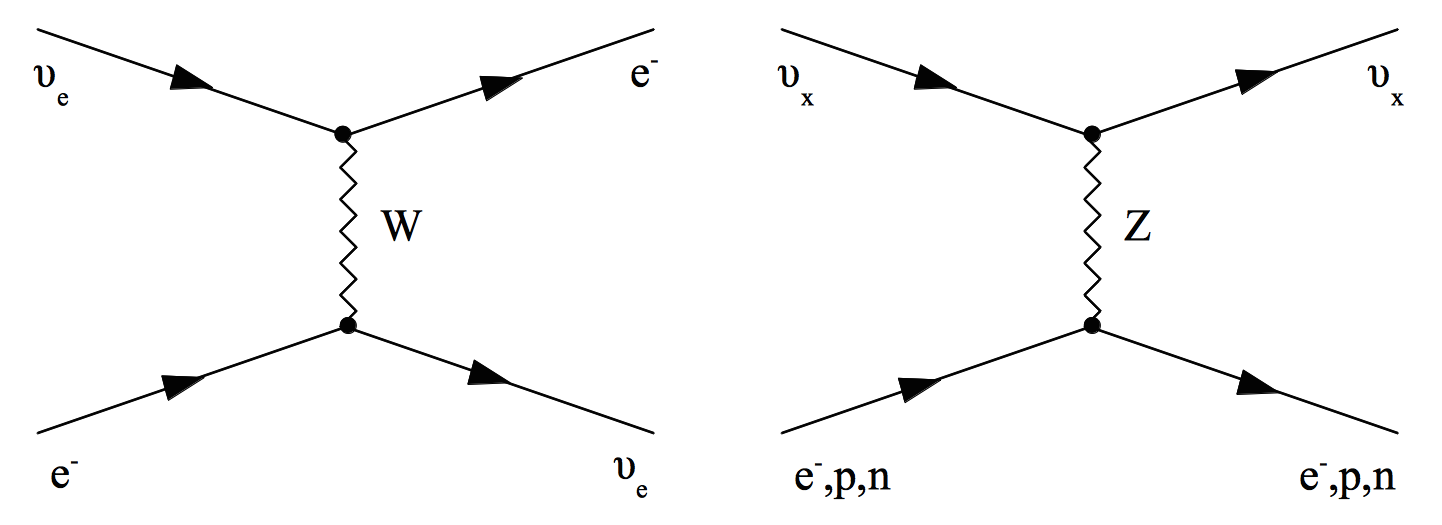
\includegraphics[width=140mm]{Introduction/IntroductionFigs/feynmanDiagramsMatterEffectsCCandNC.png}
\caption{Feynman diagrams of coherent forward scattering processes, CC on the left and NC on the right.}
\label{fig:CCAndNCFeynamnMatterEffects}
\end{center}
\end{figure}

The average effective Hamiltonian term, $\overline{{\cal H}^{(CC)}_{\textrm{eff}}}(x)$, corresponding to the CC interactions in matter is
\begin{equation}
\overline{{\cal H}^{(CC)}_{\textrm{eff}}}(x) = V_{CC}\overline{\nu_{eL}}(x)\gamma^{0}\nu_{eL}(x).
\end{equation}
Where our CC potential term $V_{CC}$ is
\begin{equation}
V_{CC} = \sqrt{2}G_{F}N_{e}
\end{equation}
with $G_{F}$ being the Fermi constant and $N_{e}$ the electron density of the medium.
The NC contribution must consider all neutrino flavour interactions with protons, neutrons and electrons.
\begin{equation}
V_{NC}^{f}= \sqrt{2}G_{F}N_{f}g_{V}^{f}
\end{equation}
Here $f$ = $e^{-}$, $p$, $n$ and $g_{V}^{f}$ is the coefficient associated with the fermion, $f$. However these coefficients are equal and opposite for protons and electrons and with electrical neutrality of atoms in matter these terms do not contribute and only the neutron term persists.
\begin{equation}
V_{NC}= -\frac{1}{\sqrt{2}}G_{F}N_{n}
\end{equation}
With $N_{n}$ as the neutron density of the medium. We then have
\begin{equation}
V_{\alpha} = \sqrt{2}G_{F}\left(N_{e}\delta_{\alpha e} - \frac{1}{2}N_{n}\right),
\end{equation}
as our total potential. Now the Hamiltonian reads, 
\begin{equation}
{\cal H} = {\cal H}_{0} + {\cal H}_{1}
\end{equation}
with our vacuum Hamiltonian term ${\cal H}_{0}$ and ${\cal H}_{1}$ arising due to the effective potential from matter effects. These matter effects are negligible in most practical cases as $G_{F} / (\hbar c)^{3} = 1.17 \times 10^{-5} $ GeV$^{-2}$, but over large enough distances through a medium, where matter densities are high, these effects can be quite considerable. Indeed such vast distances do occur in the Sun and in proposed long baseline experiments such as LAGUNA-LBNO, with the aim to use these matter effects to probe the nature of neutrinos. 

In the context of LAGUNA-LBNO, a muon (anti)neutrino beam is proposed. Both the appearance ($\nu_{\mu} \to \nu_{e}$) and disappearance ($\nu_{\mu} \to \nu_{\mu}$) channels are examined to include these matter effects. Implementing the 3 $\times$ 3 matrix the probability for the appearance transition can be approximated as equation \ref{eq:appearanceChannel} \cite{internalT2K}.
%appearance channel
\begin{eqnarray}
P(\nu_{\mu} \to \nu_{e}) & = & 4c^{2}_{13}s^{2}_{13}s^{2}_{23}\left(1 + \frac{2\alpha}{\textstyle \Delta m^{2}_{31}}(1 - 2s^{2}_{13})\right) \textrm{sin}^{2} \Delta_{31}  \notag{}\\
&& {} + 8c^{2}_{13}s_{12}s_{13}s_{23}(c_{12}c_{23} \textrm{cos} \delta - s_{12}s_{13}s_{23})\textrm{cos} \Delta_{32} \textrm{sin} \Delta_{31}\textrm{sin} \Delta_{21}   \notag{}\\
&& {} - 8c^{2}_{13}c_{12}c_{23}s_{12}s_{13}s_{23} \textrm{sin} \delta \textrm{sin} \Delta_{32} \textrm{sin} \Delta_{31}\textrm{sin} \Delta_{21}  \notag{} \\
&& {} + 4s^{2}_{12}c^{2}_{13}(c^{2}_{12}c^{2}_{23} + s^{2}_{12}s^{2}_{23}s^{2}_{13} - 2c_{12}c_{23}s_{12}s_{23}s_{13} \textrm{cos} \delta) \textrm {sin}^{2} \Delta_{21} \notag{}\\
&& {} - 8c^{2}_{13}s^{2}_{13}s^{2}_{23} \frac{\alpha L}{\textstyle 4E_{\nu}}(1 - 2s^{2}_{13}) \textrm{cos} \Delta_{32} \textrm{sin} \Delta_{31} 
\label{eq:appearanceChannel}
\end{eqnarray}

Wheres for disappearance transition probability is shown by equation \ref{eq:disappearanceChannel} \cite{georgeThesis}.
%disappearance channel
\begin{eqnarray}
P(\nu_{\mu} \to \nu_{\mu}) & = & 1 - 4s^{2}_{23}c^{2}_{13}(c^{2}_{12}c^{2}_{23} + s^{2}_{12} s^{2}_{13}s^{2}_{23} - 2c_{12}c_{23}s_{12}s_{13}s_{23} \textrm{cos}  \delta) \textrm{sin}^{2} \Delta_{23}  \notag{}\\
&& {} - 4s^{2}_{23}c^{2}_{13}(s^{2}_{12}c^{2}_{23} + c^{2}_{12} s^{2}_{13}s^{2}_{23} + 2c_{12}c_{23}s_{12}s_{13}s_{23} \textrm{cos}  \delta)  \textrm{sin}^{2} \Delta_{13} \notag{} \\
&& {} - 4(c^{2}_{12}c^{2}_{23} + s^{2}_{12} s^{2}_{13}s^{2}_{23} - 2c_{12}c_{23}s_{12}s_{13}s_{23} \textrm{cos}  \delta)  \notag{}\\
&& {} \times (s^{2}_{12}c^{2}_{23} + c^{2}_{12} s^{2}_{13}s^{2}_{23} + 2c_{12}c_{23}s_{12}s_{13}s_{23} \textrm{cos}  \delta)  \textrm{sin}^{2} \Delta_{12} 
\label{eq:disappearanceChannel}
\end{eqnarray}
Here $\Delta_{ij} = \frac{1.27\Delta m^{2}_{ij}}{eV^{2}}\frac{L}{km}\frac{GeV}{E_{\nu}}$.
In the $\nu_e$ appearance channel matter effects have been included with $\alpha = 2 \sqrt{2}G_{f}n_{e}E_{\nu} = 7.56 \times 10^{-5} eV^{2} \frac{\rho}{g / cm^{3}} \frac{E_{\nu}}{GeV}$, where the density of the earth is taken as $\rho = 2.8 g/cm^{3}$, $G_{f}$ is the Fermi constant and $n_{e}$ is the electron density \cite{georgeThesis} \cite{internalT2K}. 

Examining the expressions for the probability, the baseline $L$ and the energy $E$ are the only free parameters. Optimisation of these values and hence of $L/E$, will result in a maximal probability for the desired channel.

\subsection{Current Status}
Current values for the 3 mixing angles and the mass difference oscillation parameters have been well established \cite{oscParameters}\cite{DayaBaytheta13}, shown in table \ref{tab:osciParameterTable}.
\renewcommand{\arraystretch}{1.5}
\begin{table}[htpb]
\begin{center}
  \begin{tabular}{l*{3}{c}r}
  \hline
  \textbf{Parameter} & \textbf{Best Fit} $\boldsymbol{\pm}$ 1$\boldsymbol{\sigma}$ & \textbf{2}$\boldsymbol{\sigma}$ & \textbf{3}$\boldsymbol{\sigma}$ \\
    \hline
\hline
$\Delta m^{2}_{21} [10^{-5}eV^{2}]$ & $7.59^{+0.20}_{-0.18} $ & 7.24-7.99 & 7.09-8.19\\
$\Delta m^{2}_{31} [10^{-3}eV^{2}]$ (NH) & $2.54 \pm 0.09 $ & 2.28-2.64 & 2.18-2.73\\
$\Delta m^{2}_{31} [10^{-3}eV^{2}]$ (IH) & -($2.34^{+0.10}_{-0.09}) $ & -(2.17-2.54) & -(2.08-2.64)\\
sin$^{2}\theta_{12}$ & $0.312^{+0.017}_{-0.015} $ & 0.28-0.35 & 0.27-0.36\\
sin$^{2}\theta_{23}$ & $0.51 \pm 0.06 $ & 0.41-0.61 & 0.39-0.64\\
sin$^{2}\theta_{13}$ & $0.024 \pm 0.08 $  &  0.012-0.036 & 0.010-0.038\\
    \hline
  \end{tabular}
      \caption{The current neutrino oscillation parameters with best fit, 2 $\sigma$ and 3 $\sigma$ values, from \cite{oscParameters}, with the recent result from Daya Bay of $\theta_{13}$ \cite{DayaBaytheta13}.}
    \label{tab:osciParameterTable}
\end{center}
    \end{table}
\renewcommand{\arraystretch}{1.0}

Of the parameters in table \ref{tab:osciParameterTable} that which has been of most recent interest is $\theta_{13}$. It remained the last mixing angle to be determined and initial evidence from T2K \cite{T2Ktheta13} indicated that it had a non-zero value. More recent results are the Daya Bay $\theta_{13}$ value shown in table \ref{tab:osciParameterTable} and the even more recent result from RENO of sin$^{2}2\theta_{13} = 0.103 \pm 0.013(stat) \pm 0.011(syst)$ \cite{RENO}. These combined efforts to determine $\theta_{13}$ have shown that this parameter is no longer of key interest to future experiments and focus can be moved onto the remaining undetermined parameters, $\delta_{CP}$ and the sign of $\Delta m^{2}_{31}$.

Current global analysis of the six independent parameters, sin$^{2}\theta_{12}$, sin$^{2}\theta_{13}$, sin$^{2}\theta_{23}$, $\delta m^{2}$ $\equiv$ $\Delta m^{2}_{21}$, $\Delta m^{2}$ $\equiv$ $m_{3}^{2} - (m_{1}^{2} + m_{2}^{2})/2$ (+$\Delta m^{2}$ for NH and -$\Delta m^{2}$ for IH) and $\delta_{CP}$ are shown with their corresponding $N\sigma$ bounds in figure \ref{fig:globalNeutrinoPara1} \cite{fogliNeutrinoPlots}. The constraints of the parameters sin$^{2}\theta_{13}$ and $\delta_{CP}$ can be seen in figure \ref{fig:globalNeutrinoPara2} when examining the combination of Long Baseline (LBL) accelerator experiments, Solar experiments, KamLAND, and Short Baseline (SBL) reactor experiments and Atmospheric detectors. 

\begin{figure}[htbp]
	\begin{center}
		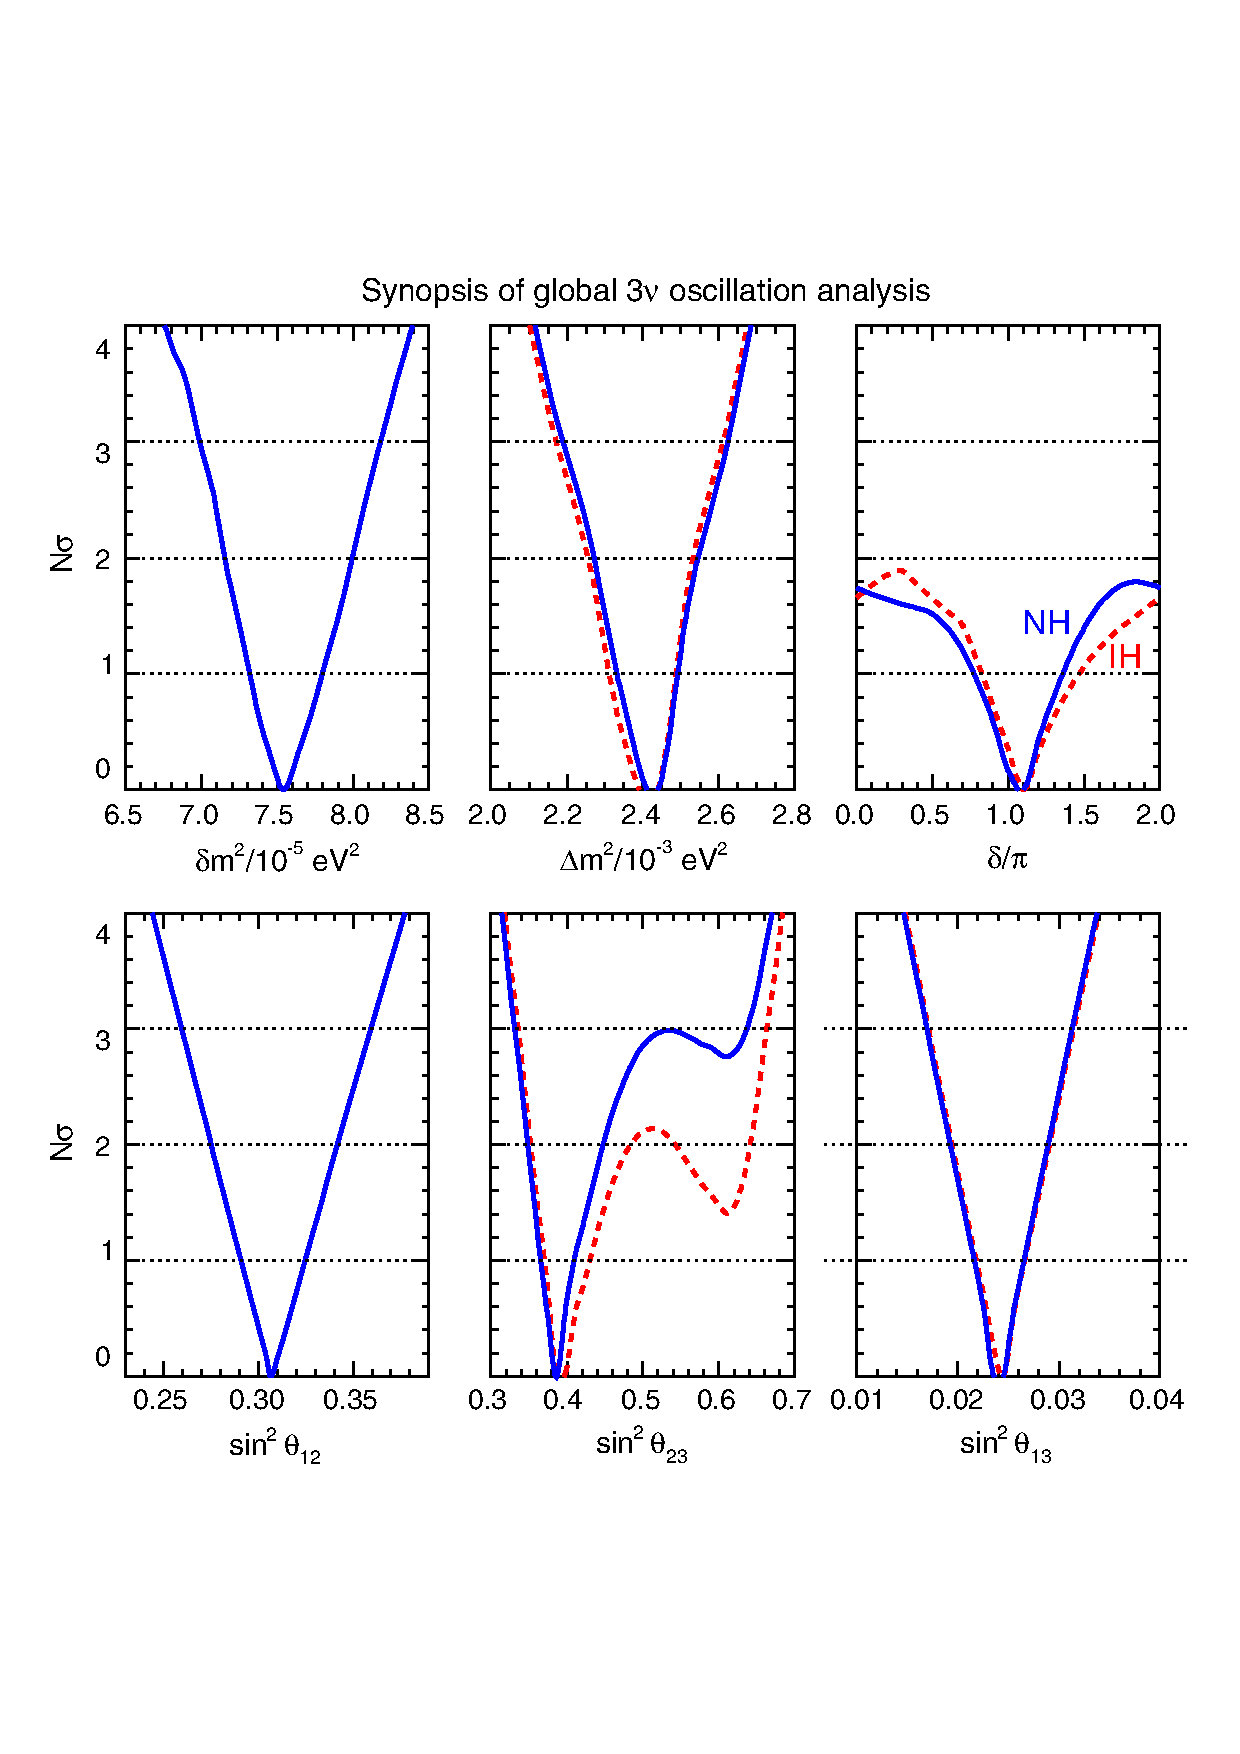
\includegraphics[width=150mm]{Introduction/IntroductionFigs/globalAnalysisNeutrinoPlots1.pdf}
		\caption{The six parameters, sin$^{2}\theta_{12}$, sin$^{2}\theta_{13}$, sin$^{2}\theta_{23}$, $\delta m^{2}$ $\equiv$ $\Delta m^{2}_{21}$, $\Delta m^{2}$ $\equiv$ $m_{3}^{2} - (m_{1}^{2} + m_{2}^{2})/2$ (+$\Delta m^{2}$ for NH and -$\Delta m^{2}$ for IH) and $\delta_{CP}$ are shown from a global analysis with their corresponding $N\sigma$ bounds, for 3$\nu$ flavour neutrinos. Blue solid lines indicate NH and red dashed lines indicate IH. Plots taken from \cite{fogliNeutrinoPlots}.}
		\label{fig:globalNeutrinoPara1}
	\end{center}
\end{figure}
\vspace{-5mm}
\begin{figure}[htbp]
	\begin{center}
		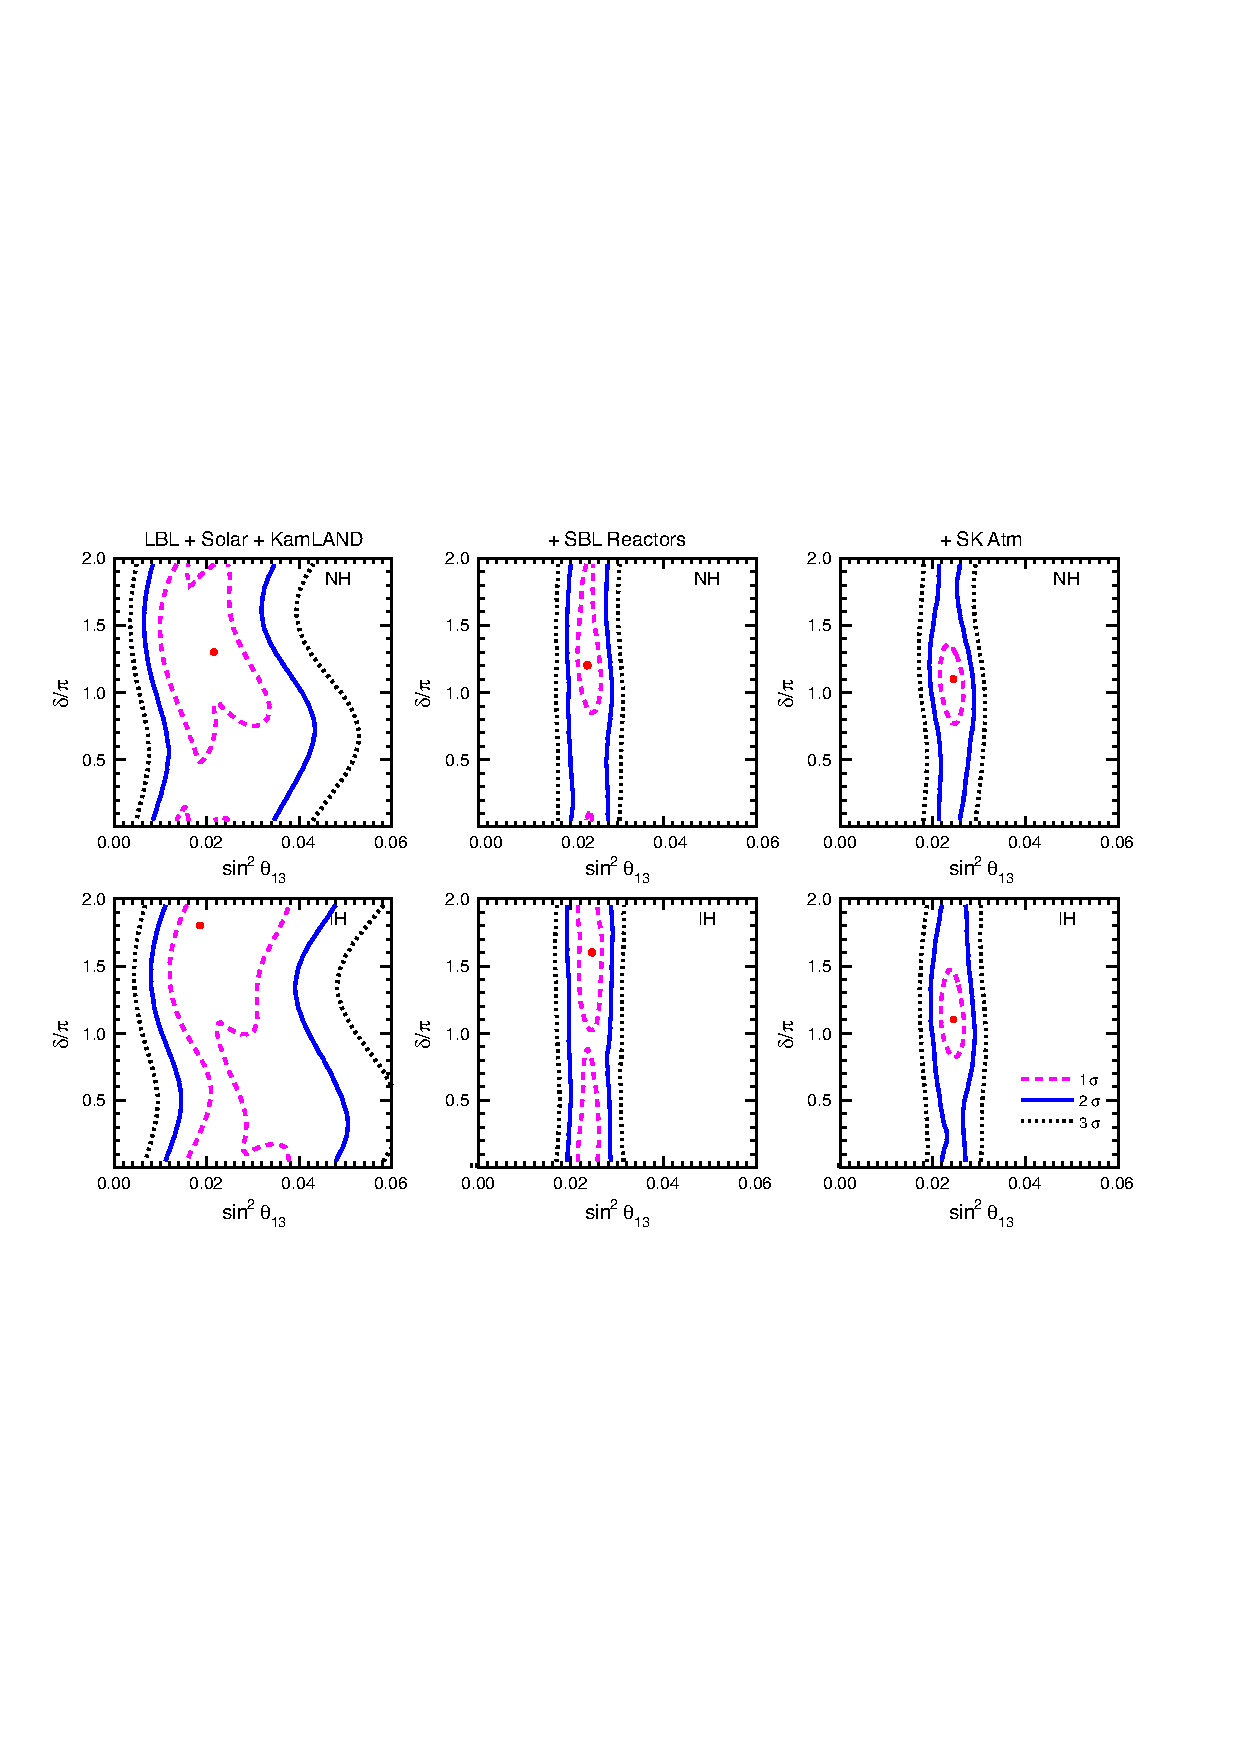
\includegraphics[width=150mm]{Introduction/IntroductionFigs/globalAnalysisNeutrinoPlots2.pdf}
		\caption{Global results in the plane of sin$^{2}\theta_{13}$ and $\delta_{CP}$. The left plots show analysis using LBL + Solar + kamLAND, the middle plots include the addition of SBL reactor experiments and the right plots include Atmospheric results. 1, 2 and 3 $\sigma$ levels are shown in dashed red, solid blue and dashed black lines respectively. Plots taken from \cite{fogliNeutrinoPlots}.}
		\label{fig:globalNeutrinoPara2}
	\end{center}
\end{figure}

\subsection{CP Violation}
From the MNSP mixing matrix there then remains one unknown parameter, the CP-violating phase, $\delta$, which can now be determined as the mixing angle $\theta_{13}$ is shown to be non zero (or integer multiples of $\pi$) to larger than 5$\sigma$. The measurement of a large $\theta_{13}$ was crucial for probing $\delta_{CP}$ as it is coupled with sin$\theta_{13}$ in the MNSP. By comparing neutrino with anti-neutrino beams in Positive Focusing (PF) and Negative Focusing (NF) run modes respectively, asymmetries in their oscillation amplitudes will show a direct observation of CP Violation (CPV) in the leptonic sector. One can define the CP asymmetry as equation \ref{eq:cpViolation}.
\begin{equation}
	A^{CP}_{\alpha\beta} = P(\nu_{\alpha} \rightarrow \nu_{\beta}) - P(\overline{\nu}_{\alpha} \rightarrow \overline{\nu}_{\beta})
	\label{eq:cpViolation}
\end{equation}

\subsection{The Mass Hierarchy}
It is clear from looking at the oscillation probabilities that they depend on $\Delta m^{2}_{ij}$ but the problem lies in the sign of these. Is $m^{2}_{3} > m^{2}_{1}$? This is a question that remains unresolved. In a vacuum these probabilities cannot discriminate between the sign as they arise in sine and cosine terms which cancel out the sign effects. However with the inclusion of the effective matter potential and the MSW effect, terms arise in the oscillation probability to make it possible to observe this sign. It is well established that $\Delta m^{2}_{21}$ is positive \cite{solarNeutrinoMassDifference}. This is due to matter effects of the Sun. 
The mass hierarchy problem is the problem of resolving  the sign of $\Delta m^{2}_{13}$, illustrated in figure \ref{massHierarchyFig}. This sign can only be determined through the appearance channel as the disappearance channel involves squared terms of the sign. 

\begin{figure}[htbp]
\begin{center}
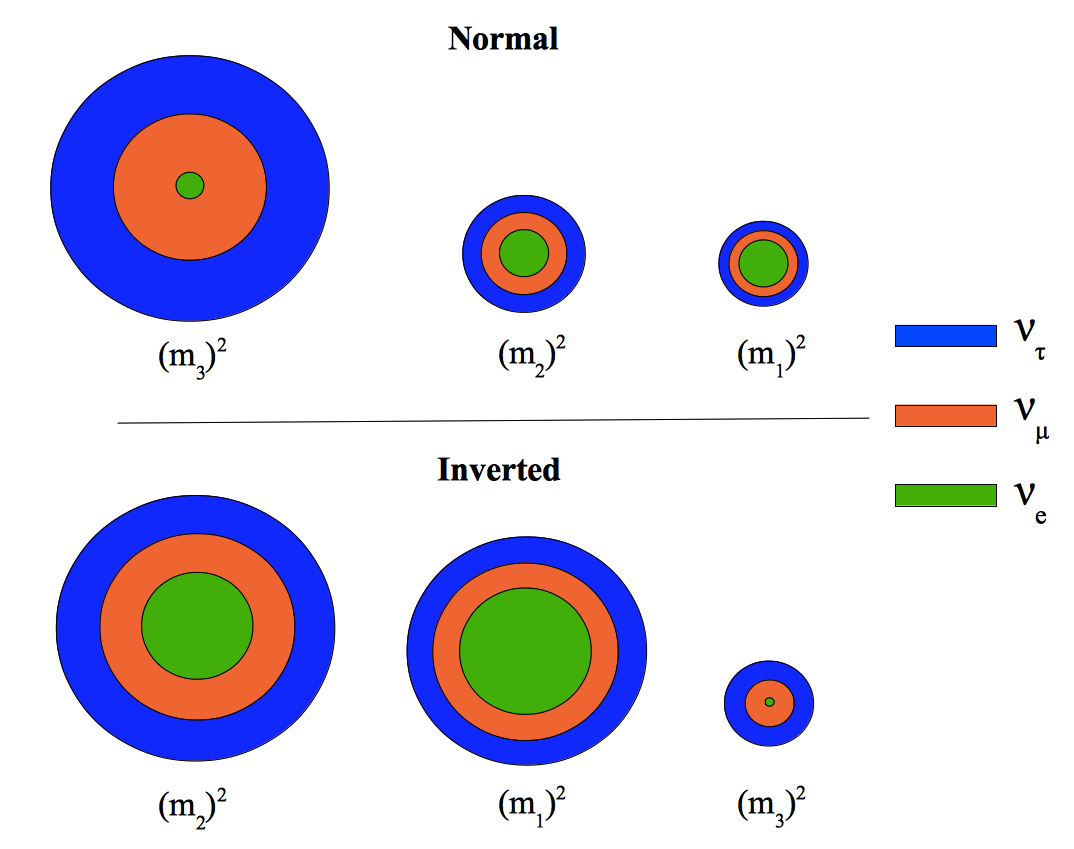
\includegraphics[width=100mm]{Introduction/IntroductionFigs/MassHierarchy_v2.png}
\caption{The mass hierarchy of neutrinos, the normal hierarchy (NH) on the top and the inverted hierarchy (IH) on the bottom. This graphic shows the larger the circle the larger the value of $m_{i}^{2}$.}
\label{massHierarchyFig}
\end{center}
\end{figure}

\subsection{Sterile Neutrinos}
Neutrinos could in theory oscillate to other flavours that do not interact weakly, unlike the 3 flavours we currently observe. This would then alter observed oscillation probabilities and could give an indirect indication to such a family of neutrinos. These particular variety of theorised neutrinos are named sterile neutrinos and as of yet are to be experimentally confirmed. 

\subsection{Neutrino Interactions}
Neutrinos can only interact in one way (ignoring gravity), that is, weakly. These interactions are well described processes in the Standard Model. Although neutrino oscillations are not described in the Standard Model, there have been no experimentally observed deviations from the Standard Model for neutrino interactions. Of course oscillations imply neutrino mass, and the Standard Model does not account for this but with neutrino mass limit $m_{\nu_{e}}$< 2.3 eV/c$^{2}$ at 95\% confidence \cite{electronNeutrinoMassTritium}, the kinematic effects of this small mass are negligible for oscillation experiments and are only relevant for mass measurement experiments.

In order to perform accurate oscillation measurements, neutrino interactions need to be well understood. LAGUNA-LBNO and most long baseline experiments are concerned in the intermediate energy scale of 0.1 to 100 GeV \cite{neutrinoCrossSections}. In this energy range several important physical process contribute. 
%It is a difficult process to accurately describe the neutrino scattering mechanisms at these energies and several models are employed to help understand these processes, mainly, nuclear, cross sectional and hadronization models. [reference her to GENIE manual]
There are three main neutrino interactions concerning this intermediate energy scale. They consist of Elastic/Quasi-Elastic (E/QE), Resonance (RES) and Deep Inelastic Scattering (DIS) interactions. 

\textbf{Elastic and Quasi Elastic:} Considered the simplest and most well understood interaction type in detectors, elastic scattering occurs with an electron or a nucleon. In either of these cases however it impossible to detect the final state neutrino in the detector and only the lepton/nucleon can be seen. 

QE interactions are not elastic but considered semi elastic due to low momentum transfer. They involve the production of new particles in the final state if above the production threshold. Charge Current Quasi Elastic (CCQE) interactions are prevalent below the $\sim$1 GeV regime, with neutrino-nucleon scatterings of
\begingroup
  \addtolength\abovedisplayskip{-0.5\baselineskip}%
  \addtolength\belowdisplayskip{-0.7\baselineskip}%
 \addtolength\abovedisplayshortskip{-0.5\baselineskip}%
 \addtolength\belowdisplayshortskip{-0.1\baselineskip}%
\begin{equation}
\nu_{l} + n \rightarrow p + l^{-},
\end{equation}
\begin{equation}
\overline{\nu}_{l} + p \rightarrow n + l^{+},
\end{equation}
\endgroup
where $l$ represents the charged lepton, $l = e,\mu,\tau$, and interacting with the proton, $p$, or the neutron, $n$ in the nucleon. In practice only electron and muon (anti)neutrinos are feasible with tau neutrino beams originating from astrophysical events. CCQE interactions are favourable in experiments as the neutrino energy can be solely reconstructed from the momentum of the lepton, by conservation of momentum and energy we have
\begin{equation}
E_{\nu_{l}} = \frac{E_{l}m_{N}c^{2} - m^{2}_{l}c^{4}/2}{m_{N}c^{2} - E_{l} + p_{l}c\cos{\theta}}.
	\label{eq:ccqeNuEnergy}
\end{equation}
Here $E_{\nu_{l}}$ and $E_{l}$ are the energies of the neutrino and lepton respectively, $m_{N}$ denotes the mass of the proton or neutron (depending on neutrino or antineutrino case). The transverse momentum of the charged lepton is given by $p_{l}$, with the angle between the lepton and the incident neutrino as $\theta$. Determination of the angle cannot be done from the lepton alone and without accurate measurement of the final state nucleons momentum it is assumed that angle is taken with respect to the beam axis. 

\begin{figure}[htbp]
\begin{center}
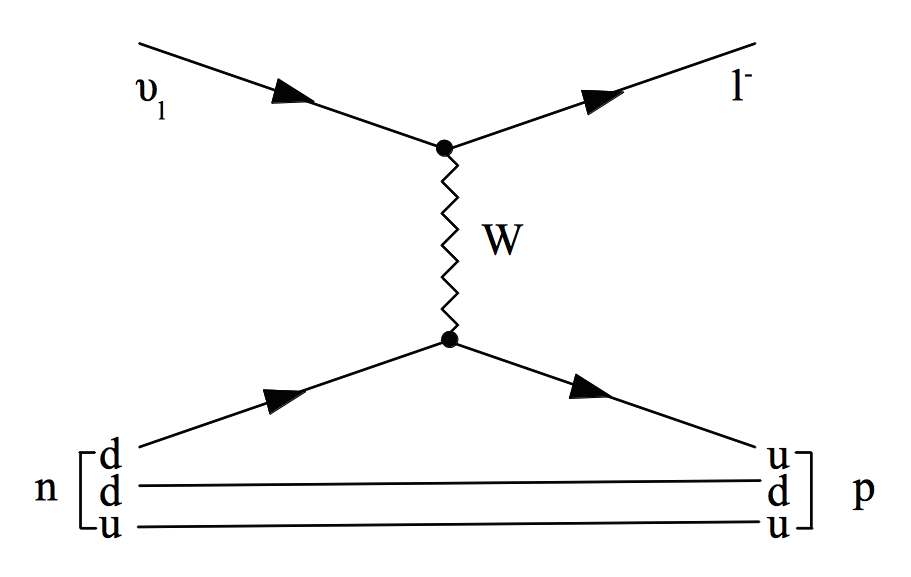
\includegraphics[width=100mm]{Introduction/IntroductionFigs/feynmanDiagramsCCQE.png}
\caption{CCQE interaction at tree level.}
\label{fig:feynmanDiagramCCQE}
\end{center}
\end{figure}

\textbf{Resonance:} In the region between elastic and inelastic processes, around 1 GeV, RES events are common. Through the excitation of baryon resonances pions are produced via,
\begin{equation}
\overset{(-)}{\nu_{l}} + N \rightarrow l^{\pm} + N^{\ast},
\end{equation}
where $N^{(\ast)}$ denotes a nucleon in a non-resonant/resonant state. The excited state $N^{\ast}$ then decays with pions in the final state.
\begin{figure}[htbp]
\begin{center}
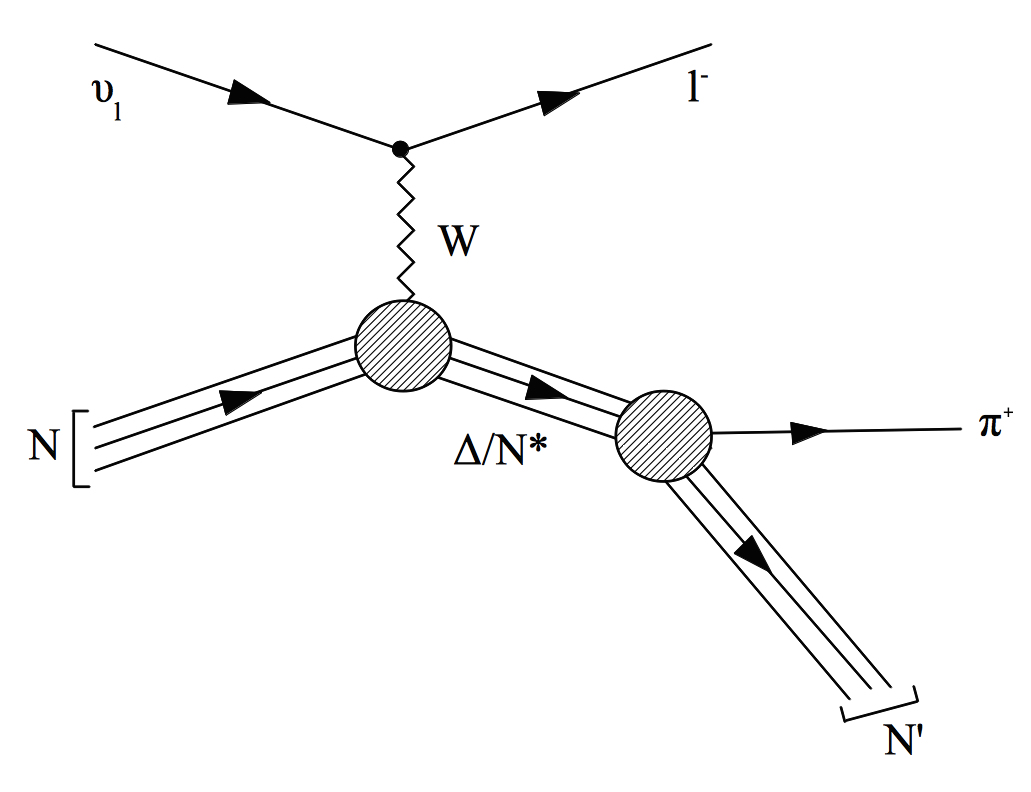
\includegraphics[width=100mm]{Introduction/IntroductionFigs/feynmanDiagramsRES.png}
\caption{RES interaction with single pion production at tree level.}
\label{fig:feynmanDiagramCCQE}
\end{center}
\end{figure}

\textbf{Deep Inelastic Scattering:} When neutrino energies are high enough that they well exceed the proton/neutron mass, $E_{\nu} >> m_{N}$, DIS interactions dominate. These processes are defined as
\begin{equation}
\overset{(-)}{\nu_{l}} + N \rightarrow l^{\pm} + X,
\end{equation}
with $N$ = proton or neutron and X represents a set of final state hadrons. Such interactions are notoriously difficult to fully reconstruct in detectors as they usually results in high multiplicities. Determining cross sections of such events require the use of structure functions, $F_{i}(x,Q^{2})$ which are given in terms of two Lorentz invariants, $x \equiv Q^{2}/2p_{N} \cdot q$ and $Q^{2} \equiv -q^{2}$ \cite{giuntiNeutrino}.

\begin{figure}[htbp]
\begin{center}
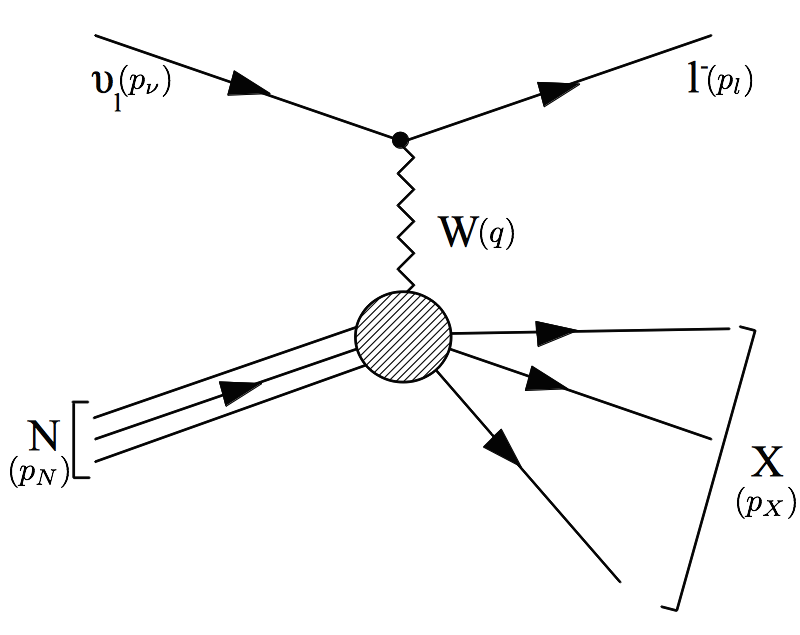
\includegraphics[width=100mm]{Introduction/IntroductionFigs/feynmanDiagramsDIS.png}
\caption{DIS interaction at tree level.}
\label{fig:feynmanDiagramDIS}
\end{center}
\end{figure}
%Neutrinos can interact with the nucleon, nucleus, individual quark in the nucleus or an electron. With this....

Quantum ChromoDynamics (QCD) and nuclear effects make understanding neutrino interactions difficult. Neutrinos can interact on the atomic scale, nuclear scale or quark scale. Due to the non perturbative nature of these interactions several models are used to describe the various interaction processes. Current experimental measurements of neutrino cross sections are not well known in the low GeV range, with several different models and calculations driving most oscillation measurements. These current measurements are shown in figure \ref{fig:nuCrossSectionsZeller} \cite{neutrinoCrossSections}. 

\begin{figure}[htbp]
\begin{center}
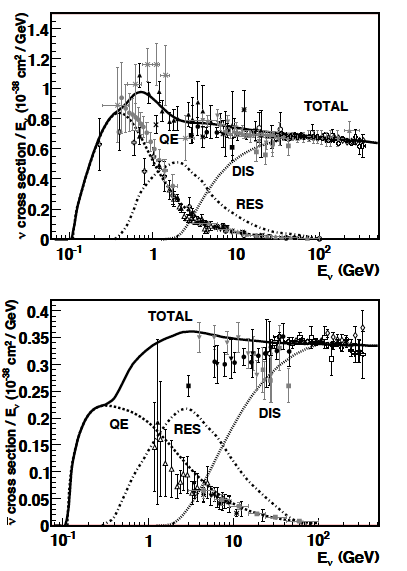
\includegraphics[width=110mm]{Introduction/IntroductionFigs/nuCrossSectionZeller2.png}
\caption{CC neutrino cross sectional data divided by neutrino energy as a function of neutrino energy for neutrino (upper) and antineutrino (lower). QE, RES single pion and DIS data is shown against predictions from an event generator. Images taken from \cite{neutrinoCrossSections}.}
\label{fig:nuCrossSectionsZeller}
\end{center}
\end{figure}

\subsection{Types of Neutrino Experiment}
Neutrino oscillation experiments can be divided into several classifications depending on their associated L/E value for the experiment. This quantity can determine the sensitivity of $\Delta$m$^{2}$, which is defined as equation \ref{eq:nuMassSensitivity} \cite{giuntiNeutrino}. The longest baseline is described first, that is neutrino experiments using the Sun as their source.

\begin{equation}
	\Delta m^{2} \sim \frac{2E [GeV]}{L [km]}
	\label{eq:nuMassSensitivity}
\end{equation}

\subsubsection{Solar Neutrino Experiments}
The Sun is a rich and powerful source of electron neutrinos due to fierce fusion processes in its core. Copious amounts of neutrinos at energies of several MeV are produced, but consist of only electron flavour, arising from reactions shown in figure \ref{fig:solarNeutrinoChain}. Large amounts of these neutrinos are produced with a neutrino flux of about 6 $\times$ 10$^{10}$ cm$^{-2}$s$^{-1}$ on the Earths surface \cite{giuntiNeutrino}. The predicted neutrino flux emitted from the Sun as a function of energy is shown in figure \ref{fig:solarNeutrinoFlux}.
\begin{figure}[htbp]
\begin{center}
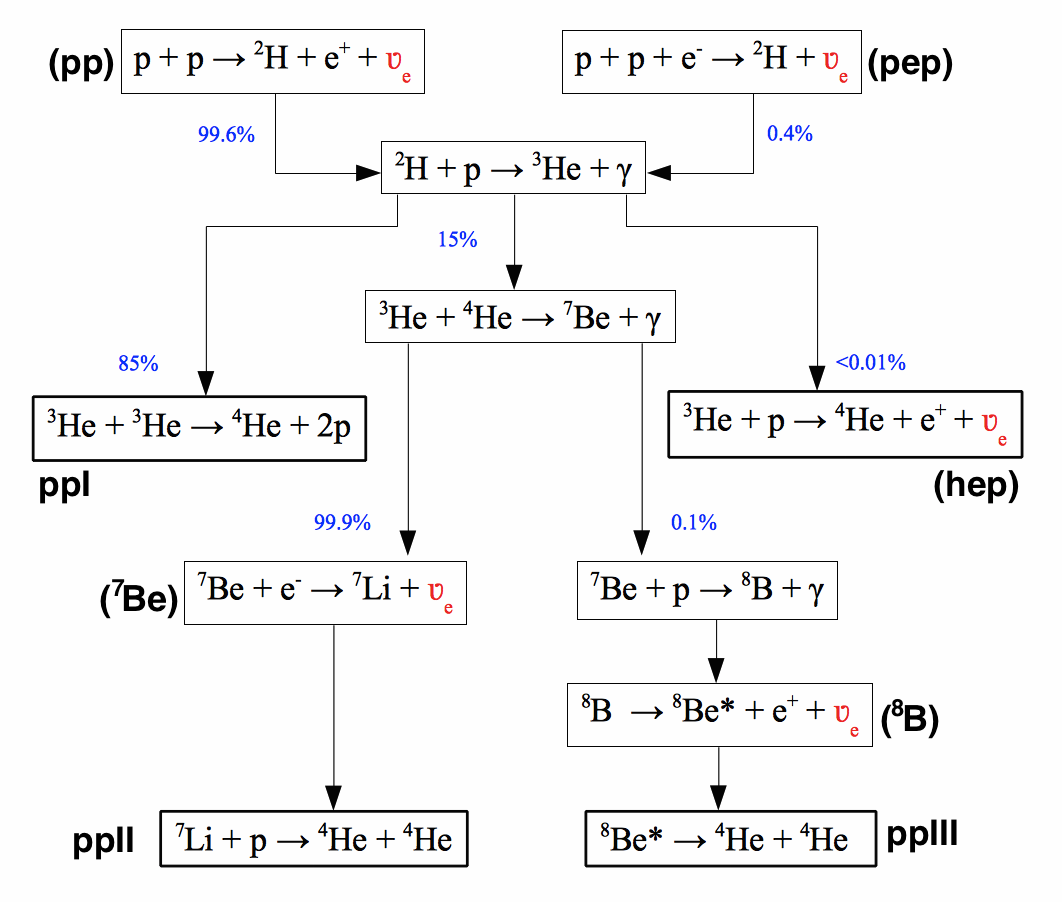
\includegraphics[width=100mm]{Introduction/IntroductionFigs/solarNeutrinoChain.png}
\caption{The fusion reactions that occur in the sun. Process chain based on \cite{giuntiNeutrino}.}
\label{fig:solarNeutrinoChain}
\end{center}
\end{figure}

\begin{figure}[htbp]
\begin{center}
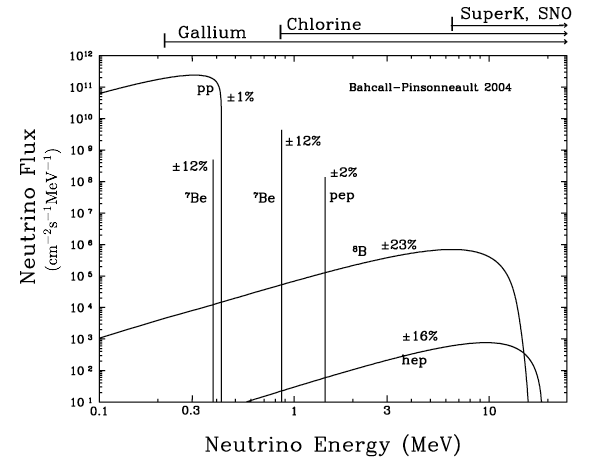
\includegraphics[width=100mm]{Introduction/IntroductionFigs/solarFlux.png}
\caption{The neutrino flux from the solar fusion processes. The percentages indicate the uncertainties in the values. Figure taken from \cite{SolarFlux}.}
\label{fig:solarNeutrinoFlux}
\end{center}
\end{figure}
The first solar neutrino experiment was the Homestake experiment conducted by R. Davis in 1968 \cite{Solar} (the origin of the Solar Neutrino Problem). Several experiments have since been conducted, providing a direct probe to the interior of the Sun. Experiments such as Kamiokande \cite{kamiokandeExperiment}, GALLEX \cite{gallexExperiment}, SAGE \cite{sageExperiment}, GNO \cite{gnoExperiment} and SNO \cite{snoExperiment} have all confirmed the Homestake observations. The latter of course resolving the Solar Neutrino problem by measuring CC interactions for the $\nu_{e}$ rate and NC interactions to yield the total $\nu$ rate.

The distance between the Sun and the Earth is approximately 1.5 $\times$ 10$^{11}$ m. With the energy spectrum ranging between 0.1 - 15 MeV this gives an upper bound of L/E $\sim$10$^{12}$ m/MeV, corresponding to a sensitivity of $\Delta$m$^{2}$ $\sim$10$^{-12}$ eV$^{2}$. Although with the radius of the Sun at roughly 7 $\times$ 10$^{8}$ m they can experience considerable matter effects inside the Sun before reaching the surface. 

\subsubsection{Atmospheric Neutrino Experiments}
Another source of naturally occurring neutrinos is from the atmosphere. Cosmic high energy particles, primarily protons, interact in the upper atmosphere producing muons, pions and kaons. These all subsequently decay into neutrinos via several different modes, with one example shown in figure \ref{fig:atmosNeutrinoDiagram}. Charged pions decay $>$99.9\% of the time via process \ref{eq:pionDecay} \cite{pionDecayModes}, producing muon (anti)neutrinos. These muons then decay via processes \ref{eq:muonDecay1} and \ref{eq:muonDecay2}. Kaons have several decay modes which all result in the production of pions, muons and neutrinos. Neutrinos of atmospheric origin have a wide range of energies varying from 500 MeV to 100 GeV.

\begin{equation}
	\pi^{\pm} \rightarrow \mu^{\pm} + \overset{(-)}{\nu_{\mu}}
	\label{eq:pionDecay}
\end{equation}
\vspace{-6mm}
\begin{equation}
	\mu^{-}  \rightarrow e^{-} + \overline{\nu}_{e} + \nu_{\mu} 
	\label{eq:muonDecay1}
\end{equation}
\vspace{-6mm}
\begin{equation}
	\mu^{+}  \rightarrow e^{+} + {\nu_{e}} + \overline{\nu}_{\mu}
	\label{eq:muonDecay2}
\end{equation}
Measurements using atmospheric neutrinos require different techniques than solar experiments as they no longer originate from one localised source. As neutrinos can originate from anywhere in the atmosphere then directional information is key in studying these neutrinos.

With distances varying dramatically depending on the several atmospheric levels, the baseline is anywhere between 10 - 10,000 km. Taking the lower bound gives a sensitivity of $\Delta m^{2} \sim$10$^{-4}$ eV$^{2}$. Kamiokande \cite{kamiokandeExperiment} and IMB \cite{imbExperiment} are two experiments that have measured atmospheric neutrinos.

\begin{figure}[htbp]
\begin{center}
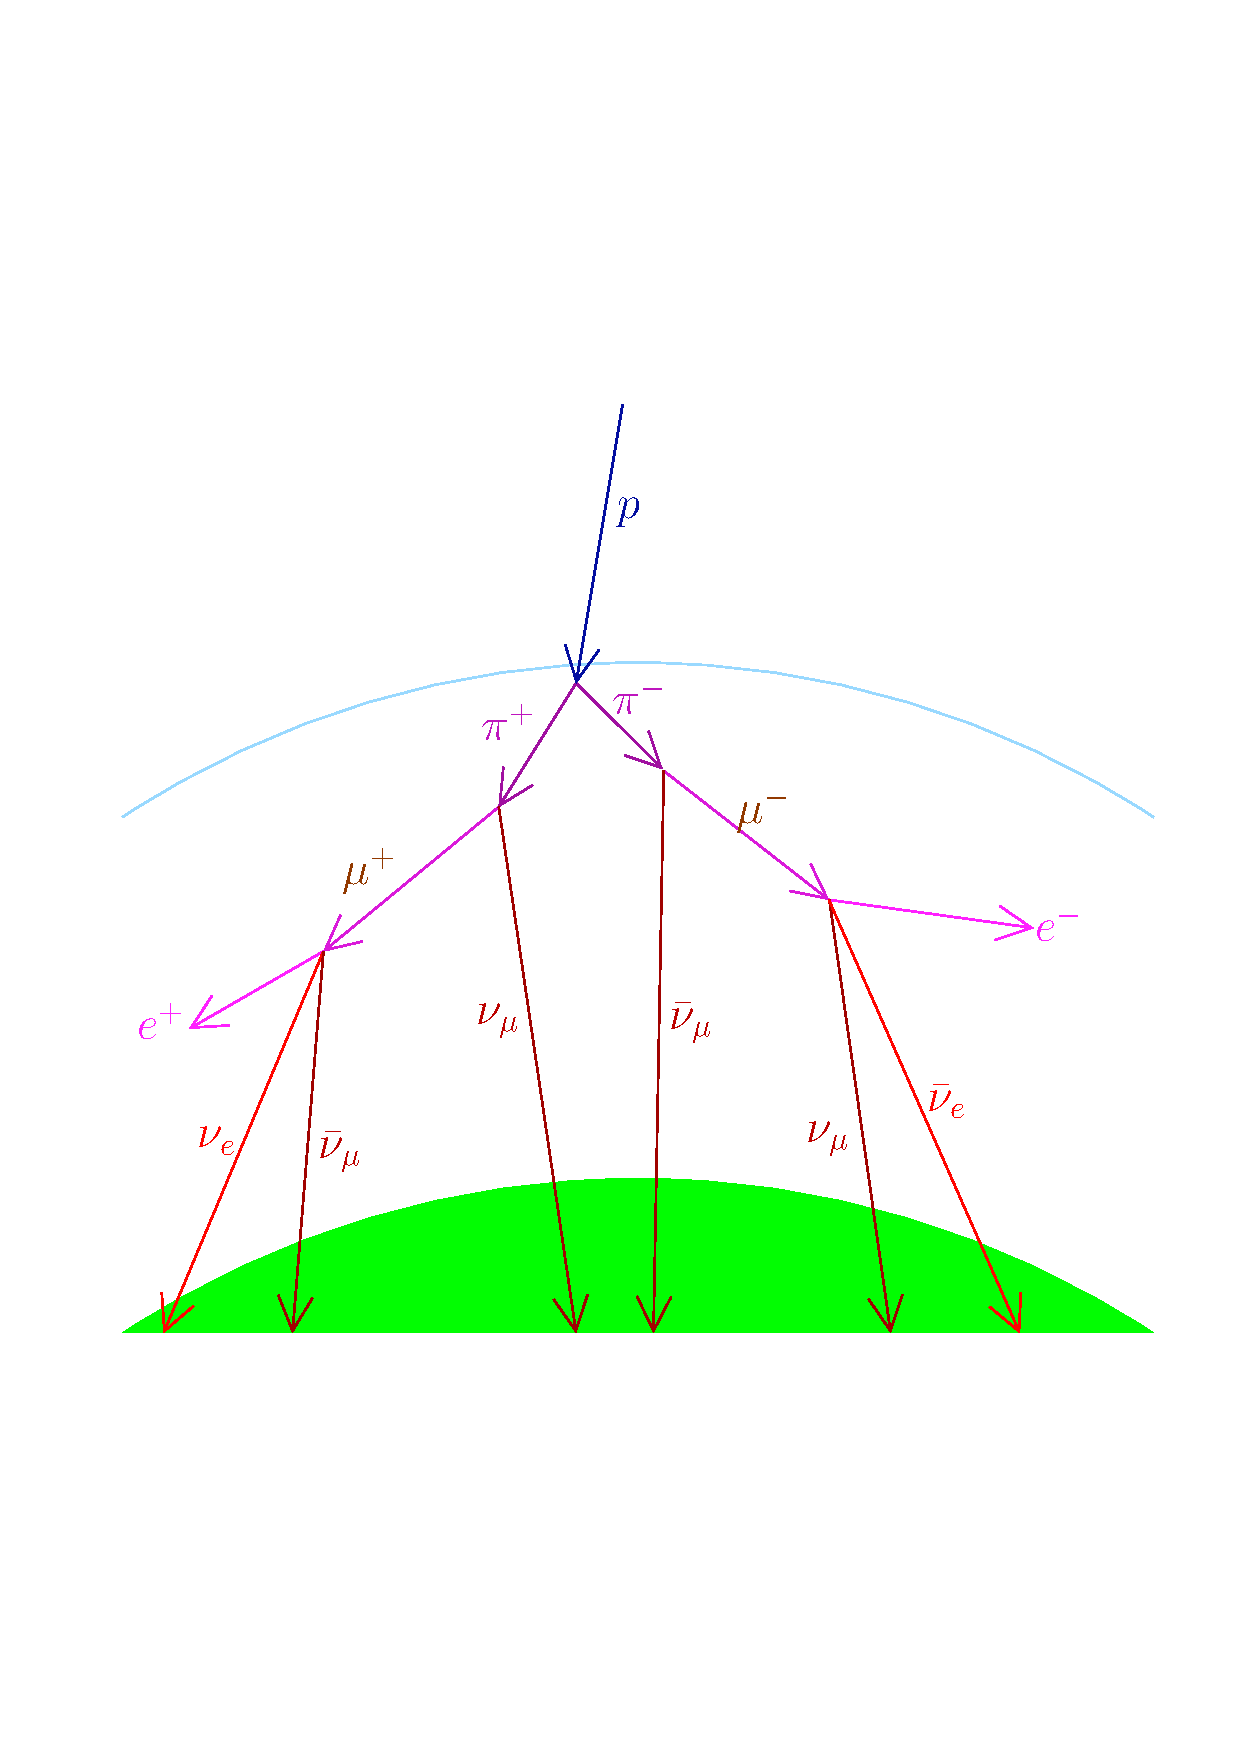
\includegraphics[width=100mm]{Introduction/IntroductionFigs/atmosNuOriginDiagram.pdf}
\caption{An illustration of how cosmic protons interact in the atmosphere and produce various flavours of neutrinos reaching the Earth's surface. Image taken from \cite{giuntiNeutrino}.}
\label{fig:atmosNeutrinoDiagram}
\end{center}
\end{figure}

\subsubsection{Reactor Neutrino Experiments}
Fission reactors are another powerful source of neutrinos, producing electron antineutrinos in large amounts $\sim$2 $\times$ 10$^{20}$ s$^{-1}$. Arising from the $\beta$-decay of fission products from reactions between $^{235}$U, $^{238}$U, $^{239}$Pu and $^{241}$Pu they have typical energies of the order of several MeV. Such energies result in shorter baselines but considering the isotropic nature of the flux this is beneficial for experiments using reactor neutrinos as a source. Only disappearance experiments are feasible as such energies are not sufficient to produce $\mu$'s or $\tau$'s in a detector through CC interactions. The common method to detect reactor neutrinos is via inverse beta decay. 

Reactor neutrino experiments can be short or long baseline, with sensitivities of $\Delta m^{2} \sim$0.1 eV$^{2}$ and $\Delta m^{2} \sim$10$^{-3}$ eV$^{2}$ respectively. Experiments that employ this method are Daya Bay\cite{dayaBayExperiment}, RENO\cite{renoExperiment} and CHOOZ\cite{choozExperiment}.

\subsubsection{Accelerator Long Baseline Experiments}
Muon (anti)neutrino beams are common in present day LBEs with the ability to perform both appearance and disappearance measurements. Neutrinos are specifically created at accelerators and aimed towards a detector at some considerable distance away, $>$10$^{3}$ km. LAGUNA-LBNO is a proposed LBE with one of the largest baselines considered in the world of 2300 km. Energies of such beams are in the regime of between 500 MeV and several GeV. At 2300 km the sensitivity to $\Delta m^{2}$ is then $\sim$10$^{-6}$ eV$^{2}$. Current accelerator LBEs are T2K\cite{t2kExperiment}, K2K\cite{k2kExperiment}, MINOS\cite{minosExperiment} and NO$\nu$A\cite{novaExperiment}.



